\xchapter{Variability analysis on public communication of emergencies}{} \label{chapter:variabilityAnalysis}

\textcolor{Escrever uma breve introdução do capítulo}

\section{Collecting Information}

We collected information on how public communication occurs during an emergency \citep{pereirachallenges} from the user organisations involved in RESCUER Project, either as official partners or as collaborators. 

To get this information, a workshop was held with the presence of representatives of Camaçari Industrial Development Committee (COFIC)\footnote{http://coficpolo.com.br/} - Brazil; the Command and Control Centre of the Public Safety \& Security Department of the State of Bahia (CICC-BA) - Brazil; and FireServ\footnote{http://www.fireserv.at/} - Austria. COFIC was in charge of providing information from the perspective of industrial parks in Brazil; CICC-BA brought the perspective of large-scale events in Brazil; and Fireserv provided information from both the perspective of industrial parks and large-scale events in Europe.

The workshop was conducted using the Brainstorm technique \citep{diehl1991productivity} and its goal was to answer the following questions:

\begin{itemize}
   \item What are the stakeholders for the public communication of emergencies?
   \item What is the relevant information in this scenario?
   \item In which emergency phases should the identified information be sent?
\end{itemize}

Furthermore, we analyse communication templates and processes provided in the partners’ manuals of security. Next, we show the results we achieved.

\subsection*{What are the stakeholders for the public communication of emergencies?}

Inside of RESCUER Project, two activities were conducted, among other things, to identify the the target audience of public communication: the Task D.1.2 Requirements Specification \citep{rescuerD11} and the Task D.4.1 Model of Organisational Behaviour and Structures in Emergencies \citep{rescuerD41}. 

Based on the list of stakeholders presented in this two tasks we elaborated an initial list of stakeholders to receive public communications: Employee / Visitor / Event Audience, Neighbouring Community, Press, and Public Authority. In addition to informing the aforementioned stakeholders, it is important to keep the public that is not directly involved in the emergency (a.k.a. General Public) informed, as this may reduce anxiety, uncertainty and prepare people for actions they should take in an emergency \citep{cdc2014}.

Workshop participants were requested to refine the initial list of public communication stakeholders, by confirming that the proposed stakeholders were relevant in real-world scenarios; detailing the list, if necessary; and informing stakeholders not covered by the initial proposal.

Workshop participants judged as necessary to replace public authority by politician and environmental department. The last is only applicable to industrial parks. The final list of public communication stakeholders is as follows:


\begin{itemize}
   \item Employee / Visitor / Event Audience (exclusive for Large Scale Events);
   \item Neighbouring Community;
   \item Press;
   \item Politician;
   \item Environmental Department (exclusive for Industrial Park);
   \item General Public.
        
 \end{itemize}


\subsection*{What is the relevant information in this scenario?}



% Please add the following required packages to your document preamble:
% \usepackage{booktabs}
% \usepackage{multirow}
\begin{table*}[]
\centering
\caption{Stakeholders x Information needs}
\label{my-label}
\begin{tabular}{@{}cccc@{}}
\toprule
\multirow{2}{*}{\textbf{\begin{tabular}[c]{@{}c@{}}Emergency-related\\ Information\end{tabular}}} & \multicolumn{3}{c}{\textbf{Stakeholder}} \\ \cmidrule(l){2-4} 
 & \begin{tabular}[c]{@{}c@{}}Employee,\\  Visitor\\ Neighbour \\  Community,\\ General Public\end{tabular} & \begin{tabular}[c]{@{}c@{}}Regulatory \\ Agency\end{tabular} & \begin{tabular}[c]{@{}c@{}}Press and \\ Politician\end{tabular} \\ \midrule
\begin{tabular}[c]{@{}c@{}}Incident Location, Incident Type, Incident Time, Taken Measures,\\ Consequences (physical, material,financial etc.) and Emergency Status \end{tabular} & x & x & x \\ \midrule
Injured People & x &  & x \\ \midrule
Fatalities (or not) & x &  &  \\ \midrule
Type of Released Chemicals &  & x &  \\ \midrule
Schedule for Press Conferences &  &  & x \\ \bottomrule
\end{tabular}
\end{table*}


In this step of the workshop, participants informed not only what information is relevant but also linked it to each of the stakeholders. 

Table \ref{stkInformacao} shows the resulting mapping. This step helped to realise that the information sent to the Press and Politicians is the same. The same was observed for
Visitor / Employee, Neighbour Community and General Public.

\subsection*{In which emergency phases should the identified information be sent?}

Workshop participants agreed that all identified pieces of information can be sent in any of the emergency phases, provided that they are confirmed information. Moreover, confirmed information can change due to the evolution of the emergency situation. 

\subsection{Variability Analysis}

% \begin{figure}
% \begin{center}
%   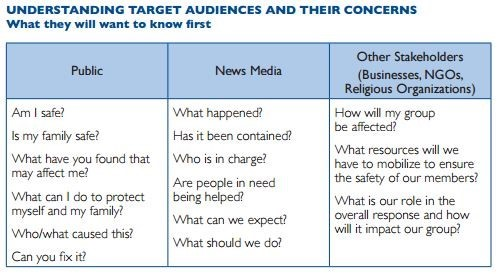
\includegraphics[width=\linewidth]{images/informationsNeeds.jpg}
% \caption{Information needs according to the target audience \citep{panamericanhealthorganization2009}}
% \label{fig:informationNeeds}
% \end{center}
% \end{figure}

The communication of an emergency varies according to the type of incident, the emergency phase and the target audience who will receive the information. The communicator needs
to provide each target audience with relevant information from their perspective, always trying to address their main concerns in a clear and objective way\citep{panamericanhealthorganization2009}. Therefore, it is essential to determine which information should be sent to each specific stakeholder, when and using which communication means.

Techniques used for variability modelling in software product line engineering can be useful for modelling commonalities and variabilities in variant-rich scenarios too. Considering the scenario of public communication of emergencies, the benefits of using variability modelling techniques are related to an efficient generation of customised messages for specific audiences, a comprehensive model to consolidate the variation points of the public communication process, and the ability to perform consistency checking of the generated messages.

% After gathering the necessary information during the workshop,  

\subsubsection{Configuration Feature Model}\label{sec:configuration}

\begin{figure}
\begin{center}
  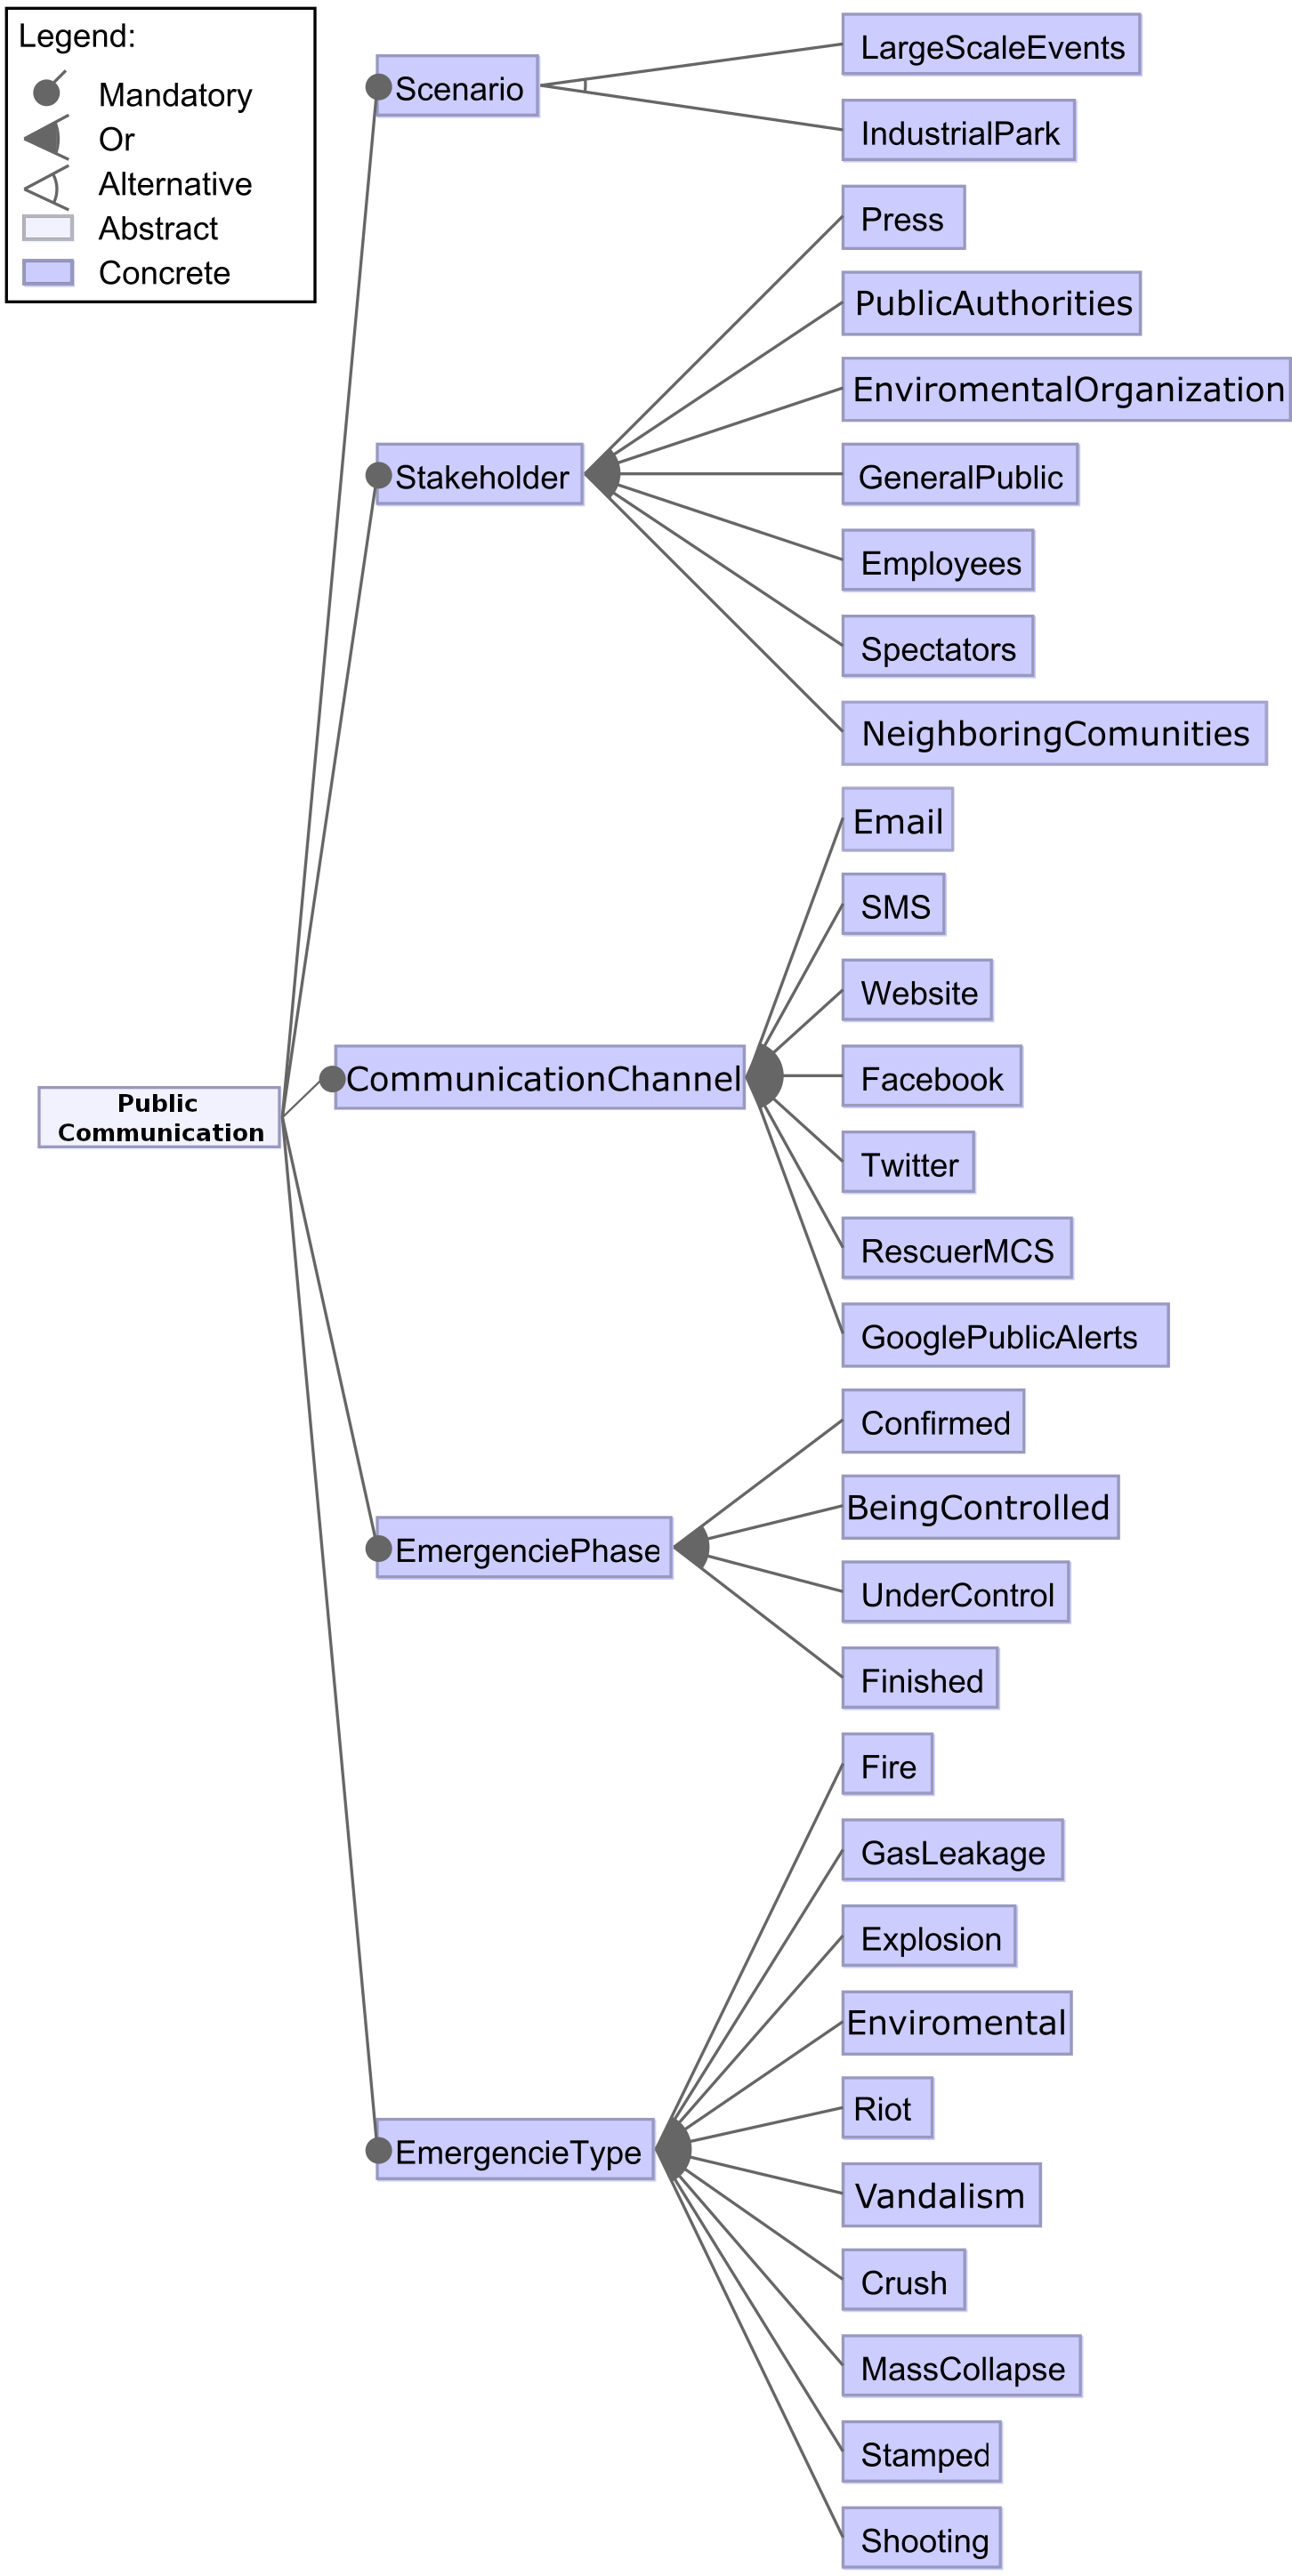
\includegraphics[width=0.75\linewidth]{images/FMConfig3}
\caption{Configuration Feature Model}
\label{fig:FMConf}
\end{center}
\end{figure}

As aforementioned, different crisis/emergency presents patterns; however, there are particularities related to the application scenarios and several other aspects. As consequence, we mapped the variation points to enable the configuration of our solution. 

Five parental features are essential to define the basic configuration of our solution: \textbf{scenario}, \textbf{stakeholder (target audience)}, \textbf{communication channel}, \textbf{emergency phase} and the \textbf{type of the emergency}. The relationship between the Scenario and its child features is ALTERNATIVE, i.e., the solution is configured for a certain organisation/scenario. Other relationships are OR (i.e., one or more sub-feature can be selected when configuring). The selection of the child features for the five parental features defines what will be possible in terms of public communication for the organisation owing the resulting configuration. Figure \ref{fig:FMConf} presents the resulting feature model.

% Please add the following required packages to your document preamble:
% \usepackage{multirow}
% Please add the following required packages to your document preamble:
% \usepackage{multirow}
\begin{table*}[]
\centering
\caption{Constraints of the configuration feature model}
\label{constraints}
\begin{tabular}{ll}
\textbf{Set of Constraints} & \textbf{Constraints} \\ \hline
\multirow{2}{*}{Scenario and Emergency Type} & Large Scale Events EXCLUDES Environmental \\
 & \begin{tabular}[c]{@{}l@{}}Industrial Park EXCLUDES Crush AND Shooting AND Riot AND Vandalism AND \\ Mass Collapse AND Stampede\end{tabular} \\
Scenario and Stakeholder & Large Scale Events EXCLUDES Environmental Organisation \\
\multirow{4}{*}{\begin{tabular}[c]{@{}l@{}}Stakeholder and \\ Communication Channel\end{tabular}} & Press or Public Authorities OR Environmental Organisations REQUIRES Email \\
 & Employees OR Neighbouring Communities REQUIRES Sms OR Rescuer MCS \\
 & \begin{tabular}[c]{@{}l@{}}General Public REQUIRES Website OR Twitter OR Facebook OR \\ Google Public Alerts OR Rescuer MCS\end{tabular} \\
 & Visitor requires Rescuer MCS
\end{tabular}
\end{table*}

Table \ref{constraints} presents the constraints that apply to the configuration feature model.

\textcolor{red}{Vaninha: Figuras e Tabelas precisam ser explicadas no texto (ainda que pareçam auto-explicativas, para promover a fluidez da leitura, e a tabela/figura ilustrar o que está sendo dito na escrita.}

There are \textbf{emergency types} that are directly related to a certain \textbf{application scenario}. For example, environmental incidents commonly are related to industrial areas, but they are not expected in large-scale events. Based on this observation, we defined two constraints to specify the valid combinations of scenarios (large-scale events and industrial parks) and emergencies types.

Likewise, we specified one constraint between \textbf{scenario} and \textbf{stakeholders}. For example, environmental organisations are not part of the target audience for any communication when the scenario is a large scale event.

The remaining constraints capture valid associations between \textbf{communication channel} and \textbf{stakeholder}. Some communication channels are more efficient to reach particular groups of stakeholders. For example, is highly unlikely that the organisation in charge of a football match in a stadium has the cell phone number or email address of visitors in order to be able to send a SMS or e-mail, but this target audience can be notified by a mobile solution based on their geographical position. Based on this observation, we present four constraints to define the set of valid associations.



\subsubsection{Variability on the Public Communication Itself}

We worked on the identification of commonalities and variabilities on the composition of public communication messages. To that end, we analyse a set of templates of our partners (COFIC and FIRESERV) and models proposed in best practice manuals \citep{cisvGuide} \citep{certTemplates} \citep{panamericanhealthorganization2009} in public communication of emergencies in order to identify the structure of this model and the relationships between their information. 

After analysing the templates, we defined a generic structure for public communications. This structure consists of the following elements: Title, Topics, Sentences and Signature:

\begin{itemize}
   \item Title: Title of the public communication;
   \item Topic: Set of sentences. Each topic has a communication goal, such as informing the occurrence of an emergency, or the actions taken to control the emergency;
   \item Sentence: Phrase (or part of a phrase) whose content can be changed by the public communicator;
   \item Signature: Complete signature of the responsible for the public communication.

 \end{itemize}
 
 First, we observed that the public communication templates change according to the current phase of the emergency. This happens because the goals of communication are different in each emergency phase \citep{cdc2014}. Another important aspect that influences the communication template is the message type. Communications channels such as social networks, SMS, and mobile applications have limitations on the message size or are used in small screens; this implies in short communication templates.
 
  \begin{figure}[]
\centering
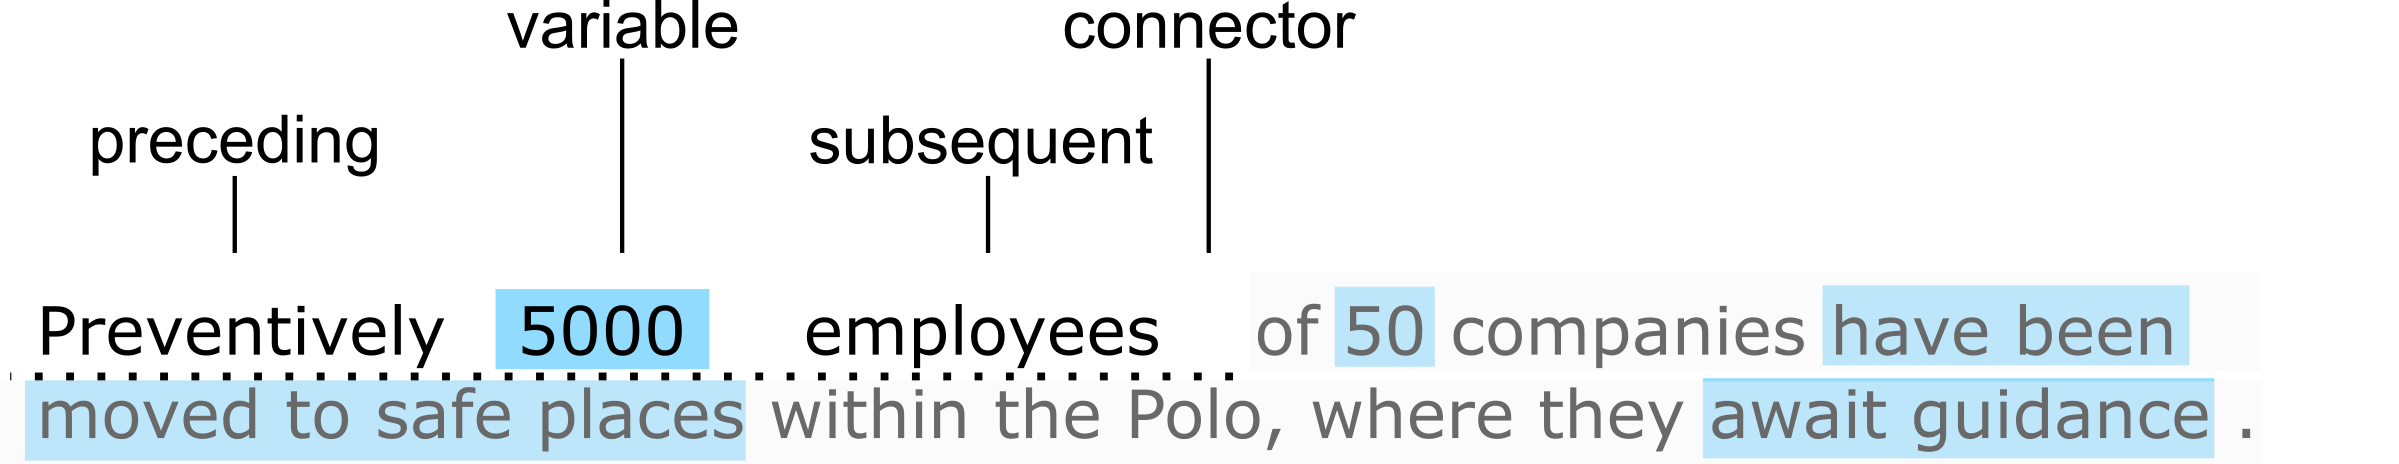
\includegraphics[width=\linewidth]{images/sentenceStructure}
\caption{Sentence Structure}
\label{fig:sentenceStructure}
\end{figure}

 
 After analysing the public communication templates, we were able to observe that sentences can be structured in: the text preceding the variable information (optional), the variable information (mandatory), the subsequent text (optional) and one connector between sentences (mandatory). Figure \ref{fig:sentenceStructure}  shows an example of connected sentences and points out the structure of one of the sentences.
 
 Furthermore, sentences are directly linked to the target audiences, as they have different concerns (Figure \ref{fig:informationNeeds}). Figure \ref{fig:FMModel} presents the result of our variability mapping of the content of public communication messages.
 
\begin{figure}[]
\begin{center}
  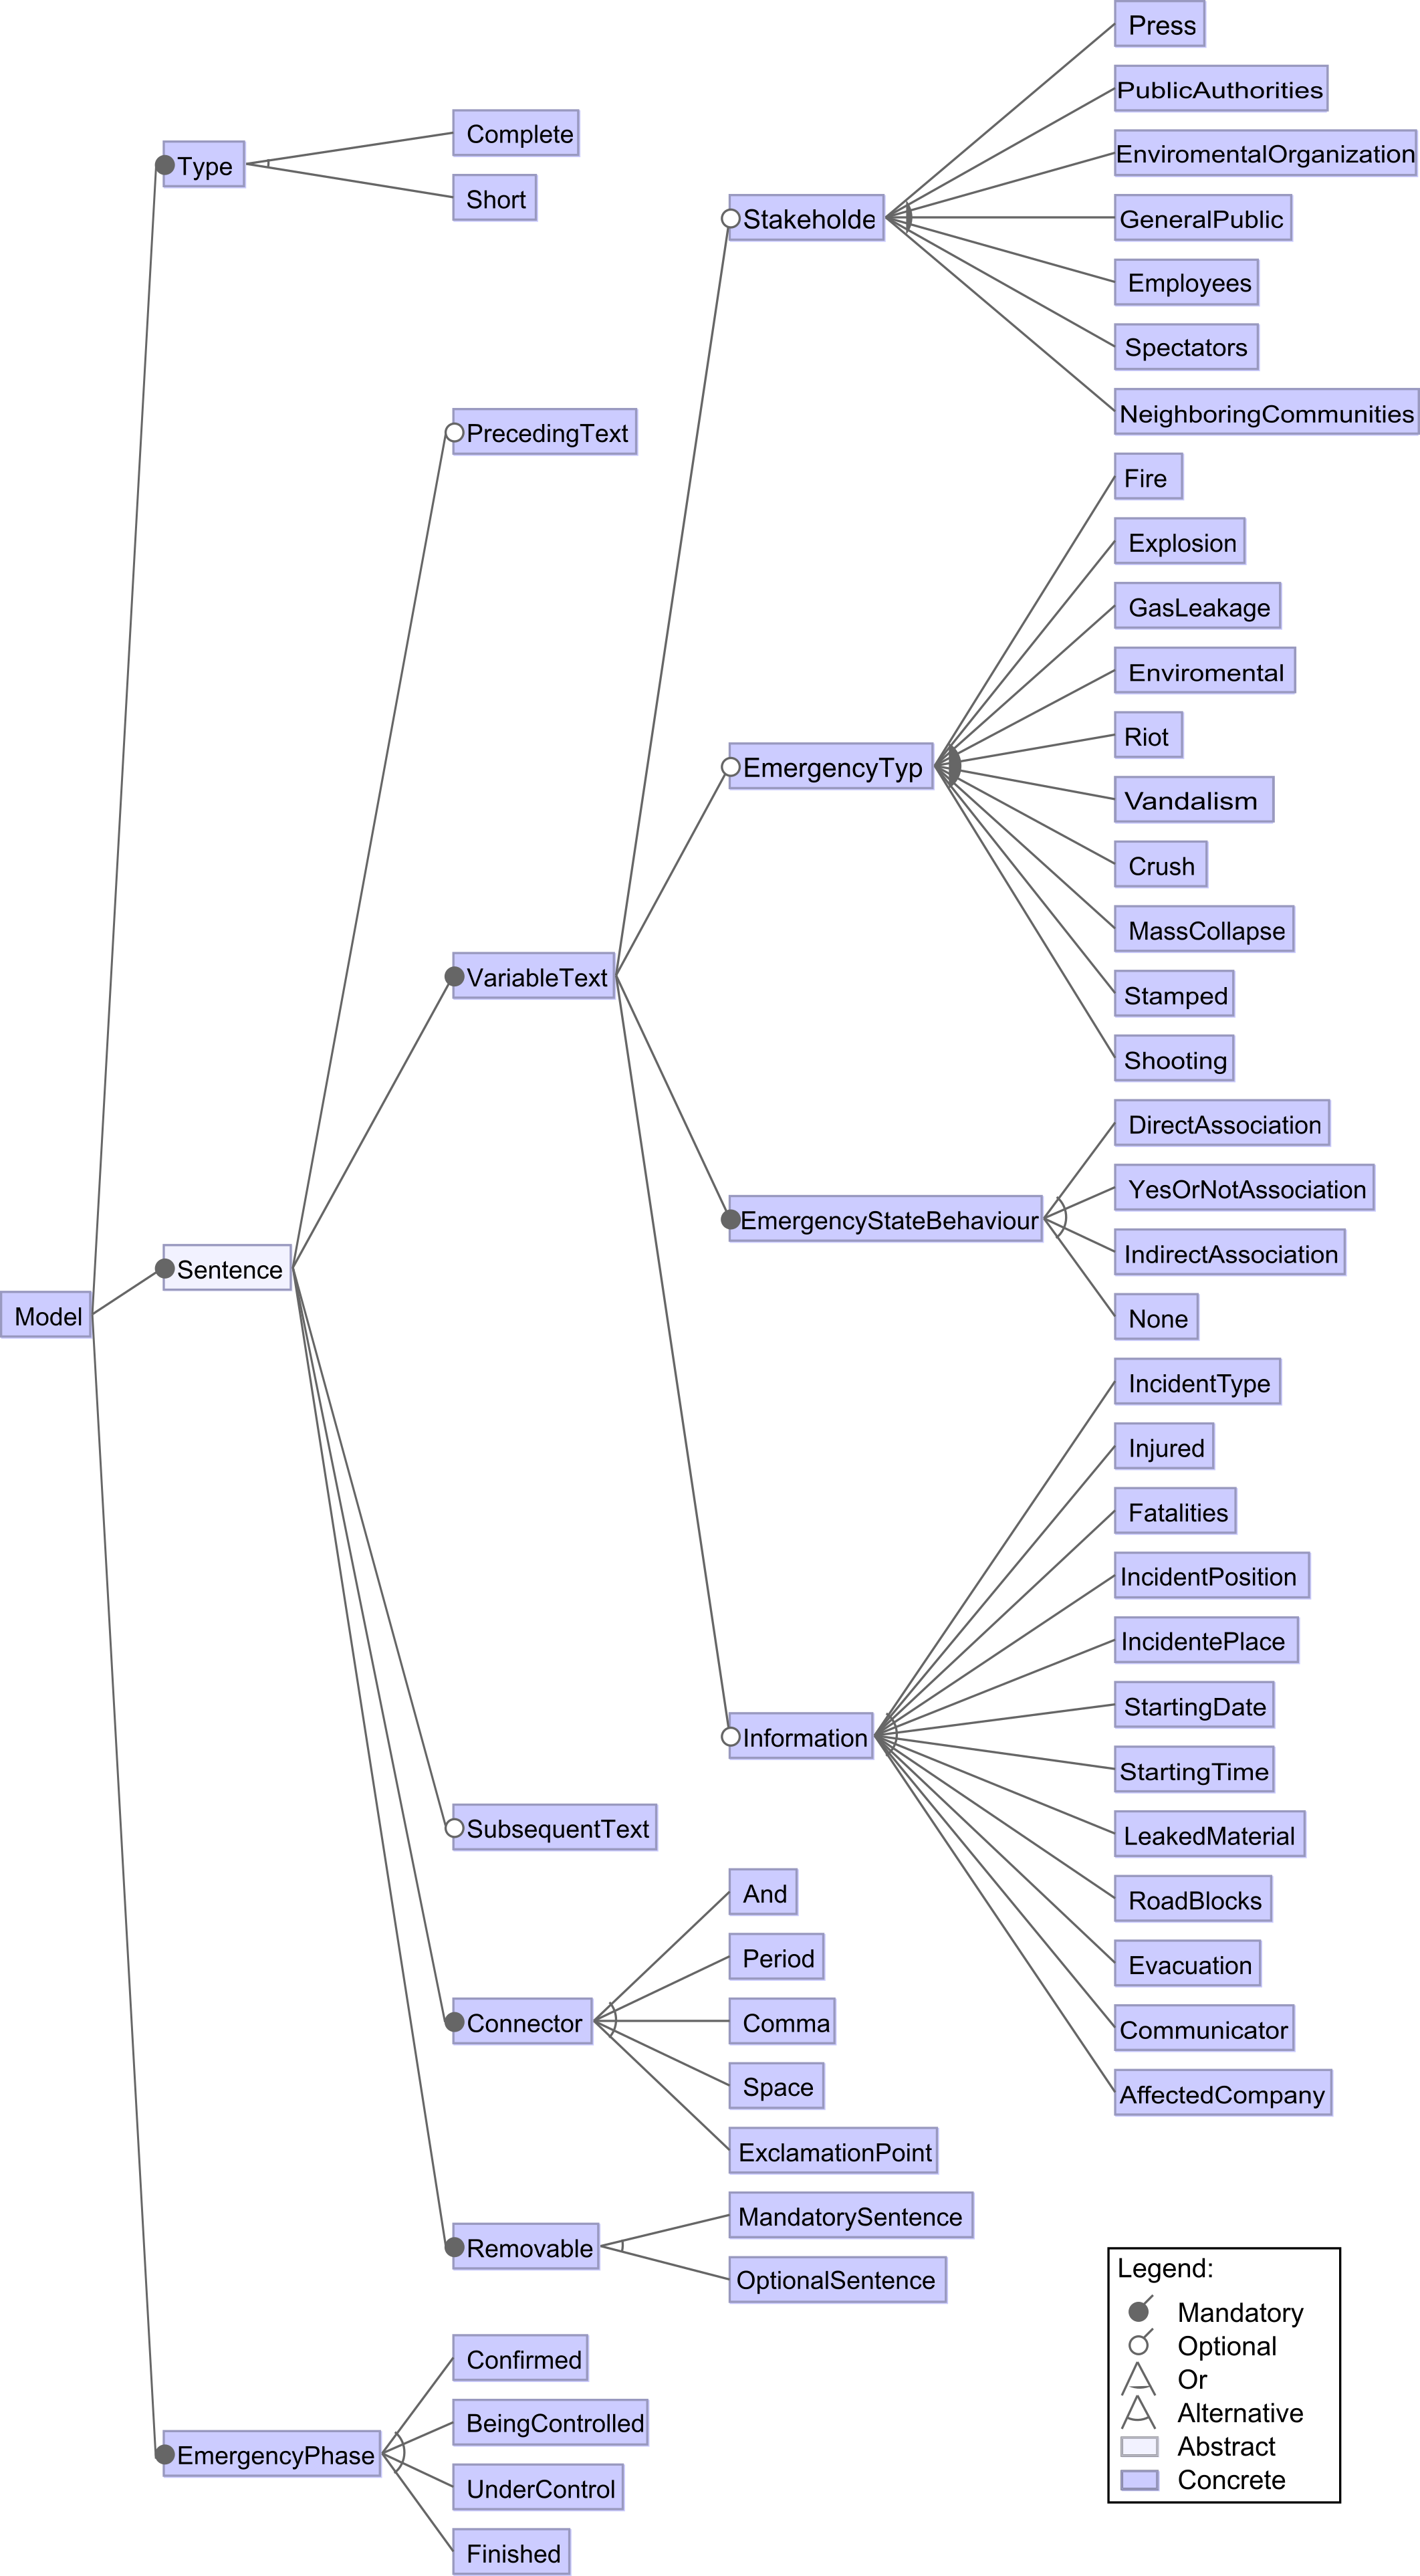
\includegraphics[width=0.75\linewidth]{images/FMModel}
\caption{Feature model for the Public Communication Itself}
\label{fig:FMModel}
\end{center}
\end{figure}